\chapter{Application on real data}
In the simulation study in the previous chapter, we contrasted the fixed intercept version and the updating intercept version of FHTBoost.
In general, FHTBoost seems to provide a decent model for correlated, realistic survival data, with average difference of deviance much smaller than 0, meaning that including covariates in the model increases its fit to test data.
We now evaluate the performance of FHTBoost on a real data example.
Specifically, we consider data from \citet{oberthuer-data}, consisting of data from patients diagnosed with neuroblastoma.
The dataset includes a relatively small number of patients, with information on two clinical covariates and around 10 000 gene expressions.
We use FHTBoost on this data to estimate an FHT model, and assess the model fit with deviance.
Finally, we compare the predictive power of FHTBoost to Cox models estimated with CoxBoost, via the Brier score (section \ref{sec:brier}), CoxBoost is a method to estimate a Cox regression model using a boosting framework (see, e.g., \citet{BinderSchumacher2008}).
We first give a description of the data set.

\section{Description of the neuroblastoma data set}
We consider survival data from \citet{oberthuer-data}, consisting of patients diagnosed with neuroblastoma.
Neuroblastoma is a malignant pediatric tumor that accounts for about 8\% of all childhood cancers.
One of the hallmarks of the disease is its contrasting biological behavior, which results in diverse clinical courses ranging from spontaneous regression to rapid and fatal tumor progression despite intensive treatment.
In recent years, several markers have been reported to offer valuable prognostic information.
These markers are routinely determined by the current German neuroblastoma clinical trial NB2004 to stratify patients into groups of high risk (50\%) or low risk (50\%) of disease.
Therapeutic strategies vary according to these risk categories, and they range from a wait-and-see approach for those in the low risk group
to intensive treatment for the high-risk group.
The risk categories are no silver bullet for predicting survival.
On the contrary, common clinical experience suggests that such risk classification is still suboptimal for a substantial number of patients.

Originally, the data consist of two separate data sets:
A larger training set, collected in Germany, and a smaller test set, collected in several countries.
The training set consists of 256 patients of the German Neuroblastoma Trials NB90-NB2004, where the patients were diagnosed between 1989 and 2004.
The test set is an independent set of 120 patients from national trials in several countries (including 29 from Germany).
Due to a low number of events in the NB2004 low risk group, and following \citet{bovelstad2009}, we merge the ``training set'' and the ``test set'' into one data set.
Hence, in total, the data consists of 362 patients suffering from neuroblastoma.
There are 9978 gene expressions measurements, comprised of those measurements that are in probes from both the ``training set'' and the ``test set.''
From each patient, we have information on their risk group according to the current German neuroblastoma trial, as well as the patient's age at diagnosis.
In this data set, 89 out of the 362 observations have missing values.
We remove all of these observations, and are left with a data set of 273 individuals with full observations.
Finally, for each individual we have the possibly censored event time, which in the case of an event is the time to a fatality, in years from diagnosis.
The median follow-up time without a fatal event was 4.14 years.
42 of the 273 children experienced a fatal event within the follow up, which is a proportion of 31.5\%.
Of these, 86 children were classified as having high-risk, while the remaining 187 were not.
The risk indicator is coded as a binary variable, where low risk is coded as 0, and high risk as 1.
We will now briefly discuss the models we intend to estimate on this data set, and how we will evaluate their performance.

\section{New models}
\subsection{Clinical-only and genetic-only FHT models}
\citet{bovelstad2009} analysed the neuroblastoma data and compared different statistical methods to combine clinical and genomic data in Cox models.
As mentioned in subsection \ref{subsec:FHT-combine}, the FHT model lends itself easily to combining genomic and clinical data, and this holds for FHTBoost as well.
There is also a straightforward way to only use one kind of covariates, i.e., only clinical covariates or only genetic covariates.
In other words, we make a genomic version of FHTBoost, or $y_0$-only version of FHTBoost, by only boosting the initial level $y_0$.
Similarly, we make a clinical version by not letting $y_0$ depend on covariates, i.e., let $\X$ be empty.
In this way, we can compare the performance of our model across the genetic and clinical data, in a similar way as in \citet{bovelstad2009}.

\subsection{Boosted Cox model}
To properly assess the predictive power of our estimated FHT models, we need to compare it to state of the art methods.
As we have discussed the Cox model earlier (see subsection \ref{subsec:ph-reg}), and we have implemented a boosting algorithm for the FHT model, we find it appropriate to use \textit{CoxBoost} \citep{coxboost}.
It is an R package for estimating boosted additive predictors for the Cox model.
There exists a gradient boosted Cox estimation method in \textit{mboost}, but its cross-validation procedure in was broken at the time of this thesis. 
\textit{CoxBoost} uses likelihood based boosting \citep{gamboost}, which is a similar boosting method that arrives at very similar Cox estimates.
In likelihood boosting, the tuning parameter is $\lambda$, and while it is not directly comparable to the step length $\nu$ in gradient boosting algorithms, we set
\begin{equation}\label{eq:lambda-nu}
    \lambda=\frac{N(1-\nu)}{\nu},
\end{equation}
as suggested in \citet{DeBin2016}.
The size of $\lambda$, like the step length in gradient boosting, is not very important.
As long as it is roughly the appropriate size, it does not have a large effect on parameter estimates.
Here $N$ is the number of individuals in the data set on which the estimator is applied, and $\nu$ is the step length mentioned in the various boosting algorithms in Chapter \ref{ch:boosting}, which we by convention always set to 0.1.

In the Cox model, we include all covariates when modeling the hazard function, i.e. for this neuroblastoma data set it estimates a model of the form
\begin{equation*}
    \hat{\boldeta}_{\text{CB}}=\underbrace{\hat{\beta}_{1,1}\x_1+\hat{\beta}_{1,2}\x_{2}}_{\text{clinical}}+\overbrace{\hat{\beta}_{2,1}\z_1+\ldots+\hat{\beta}_{2,9978}\z_{9978}}^{\text{genomic}},
\end{equation*}
since there are two clinical covariates and 9978 genomic ones.
In the standard boosted Cox model, all parameters are estimated in a penalized manner.
Thus there is a chance of the clinical data not being included in a final estimated model, like for FHTBoost.
A gene covariate will not be treated any differently than a clinical covariate, but that is something we may want, as our FHT model does treat them differently.
There is also an option in \textit{CoxBoost} for specifying mandatory covariates.
These covariates will not be penalized, and hence they will be included in the final model.
We therefore in this chapter, in addition to the regular CoxBoost model, estimate a mandatory CoxBoost model, where we treat clinical covariates as mandatory.
To estimate the survival probabilities given these models, we use the method discussed in subsection \ref{subsec:cox-surv-prob}.
We now discuss the results from one split of the data into training and test sets.
Finally, note that we did not verify that the proportional hazards assumption is true for this data, so although the performance may be good, the theoretical assumptions may not hold in this case.

\section{A single split of the data set}
Due to the lack of data, \citet{bovelstad2009} generated 50 random splits of training and test sets from the merged data set.
We do the same, only we generate 100 random splits.
This gives a more accurate estimate of the model performance, as we average out some of the variance which arises from splitting a data set of with a small sample size.
First, however, we report the analysis of one single (the first) split of train and test data, to show how to interpret the results.
The data are split in a training set (2/3) and test set (1/3), stratified by the event status.
The training set consists of 182 patients, where 28 are observed events.
The test set consists of 91, where 14 are observed events.
As usual, we estimate the models on a training set, and evaluate their performance on a test set.

\subsection{Cross-validation on training set}
As has been shown previously, cross-validation should be repeated with different division of folds, as this reduces variance in the estimator of $\mstop$.
We therefore perform a (10 times) repeated 5-fold cross validation to find the optimal number of iterations.
The resulting test errors are shown in Figure \ref{fig:neuroblastoma-cv}.
In this example the boosting algorithm, in contrast to the original AdaBoost, eventually overfits, so it is important to select the number of boosting steps by cross-validation.
Note the impact of running the cross-validation in a repeated fashion:
Each dotted gray line in the figure is the sum of the negative log-likelihood of a model trained on 4 folds and applied to the last fold, as a function of the iteration number $m$, i.e. the cross-validated test error.
We would not have selected the same $\mstop$ in all of these 10 single 5-fold cross-validations, because the minimizing $m$ for each line ranges from 22 to 50.
The solid black line is the mean of these 10 gray lines, and it is this line that we choose the minimizer of.
We find $\mstop=27$ to be optimal, i.e., the minimizing iteration number, shown as the red vertical line in Figure \ref{fig:neuroblastoma-cv}.
We run the FHTBoost algorithm with a fixed intercept for $\mstop$ iterations, resulting in an estimated model.
We first examine the model parameters.

\begin{figure}
\caption{
    Repeated 5-fold cross validation on training set generated from neuroblastoma data set \citep{oberthuer-data}.
    The grey lines refer to the cross validation error for a single 5-fold CV implementation,
    the black line is the average of 10 such replications.
    The red vertical line highlights the best value for the number of boosting steps.
}
\label{fig:neuroblastoma-cv}
\centering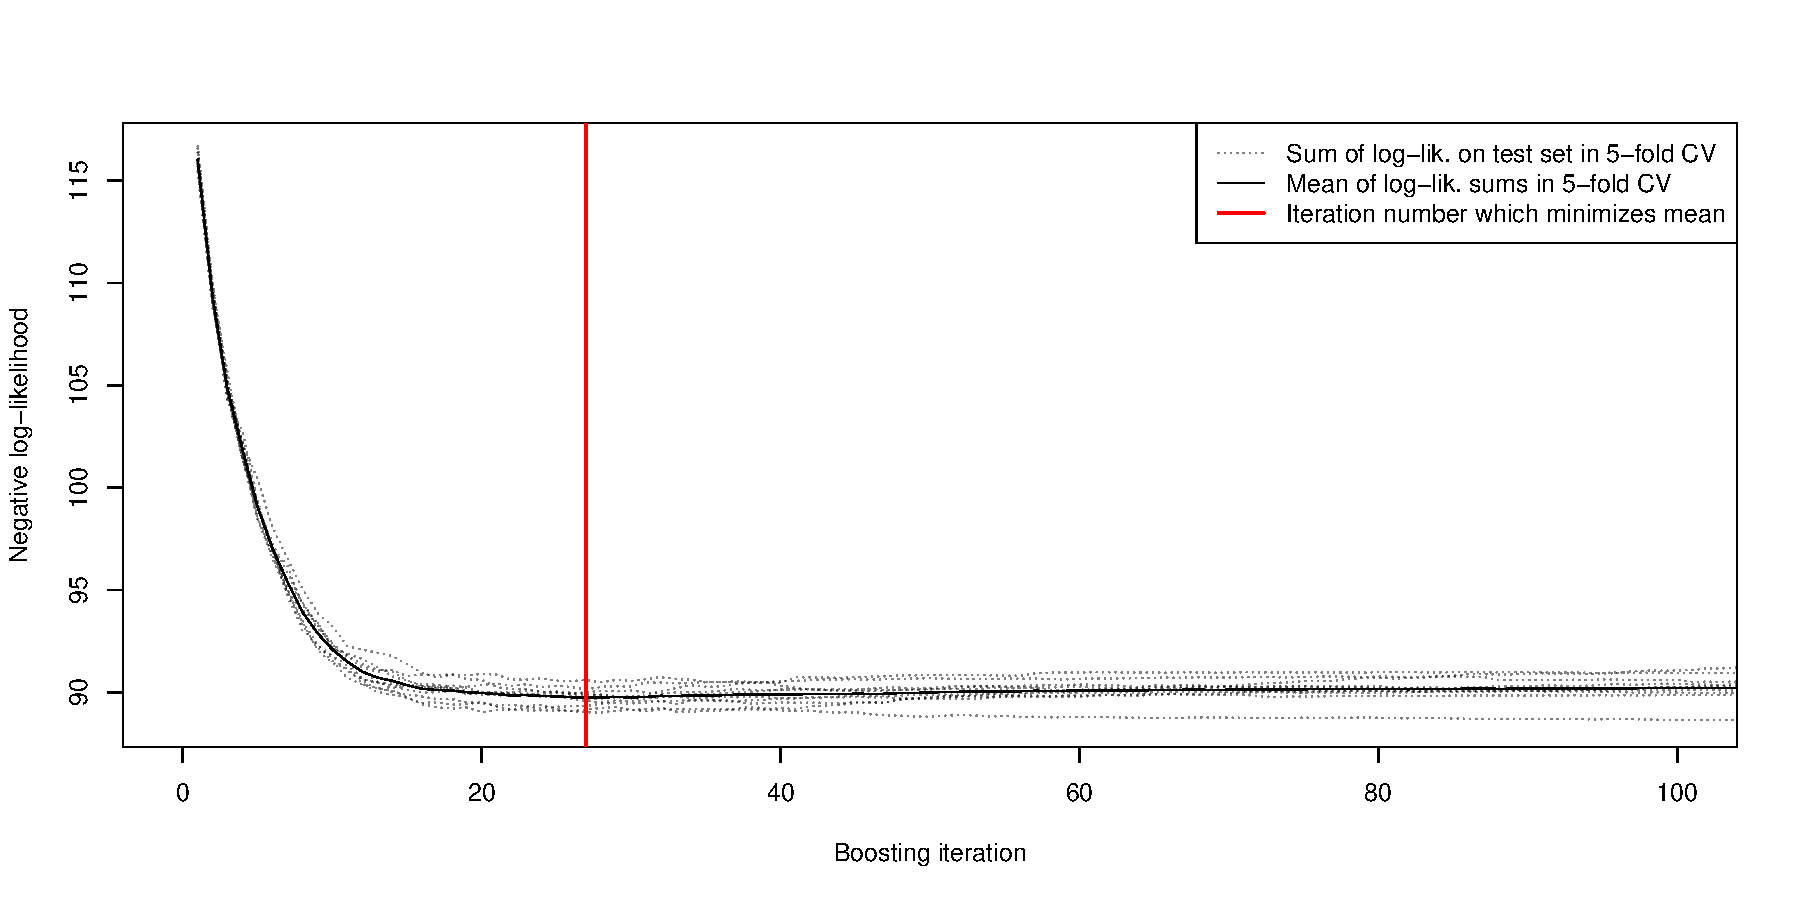
\includegraphics[scale=0.4]{example_cv_loglik_new.pdf}
\end{figure}



\begin{table}
\caption{FHT null model additive predictors estimated on a single split of the neuroblastoma data set \citep{oberthuer-data}}
\label{tab:neuroblastoma-intercepts}
\centering
\begin{tabular}{lr}
\toprule
Intercept  & Value\\
\hline
$\hat{\beta}_0$  & 0.666 \\
$\hat{\gamma}_0$ & 0.332 \\
\bottomrule
\end{tabular}
\end{table}

\subsection{Interpretation of estimated null model}
In an FHT context with a Wiener process, a null model, i.e. without covariates, means a model with initial level
\begin{equation*}
    \hat{y}_0^{[0]}=\exp\left(\hat{\beta}_0\right)
\end{equation*}
and drift
\begin{equation*}
    \hat{\mu}^{[0]}=\hat{\gamma}_0.
\end{equation*}
Note that since we are using the fixed intercept version of FHTBoost, the null model will be the same for the three types of the FHT model we are considering here.
The estimated intercepts are reported in Table \ref{tab:neuroblastoma-intercepts}.
The estimated intercept for the gene data, $\hat{\beta}_0$, is 0.666.
Remember that the vector $\bbeta$ corresponds to the initial level $y_0$ of the health process, through the log link function.
The null model, without any covariate effects, therefore has a $y_0$ of $\exp(0.666)=1.946$.
The intercept $\gamma_0$ corresponding to the clinical data is estimated to be 0.332.
Since these are related by identity link, the drift $\mu$ is also 0.332.
This means that the health process with the FHT interpretation that arises from our estimation is a Wiener process with a relatively small initial level of 1.946, and with a positive drift of 0.332.
Since we are looking at when, if ever, a neuroblastoma patient will have a fatal event after diagnosis, a relatively small initial level of the Wiener process makes sense.
It is the health level of a patient \textit{at} its diagnosis.
The health of such a child is presumably quite precarious, as neuroblastoma is a malignant cancer.
It also makes sense that the drift $\mu$ is positive, as this means the health level of a child will on average increase after it is diagnosed.
Since the individuals in the study are young children, and we are looking at a timeframe that does not comprise the length of a typical human life, the health level of most children should indeed increase after diagnosis.
We recall from section \ref{subsec:wiener} that a Wiener process $W(t)$ has variance equal to its time $t$.
The large variability of the process relative to its starting point means there is still a chance of dying of the cancer.
The resulting health process is
\begin{equation*}
    Y(t)=1.946+W(t)\cdot0.332t,
\end{equation*}
where $W(t)\sim N(0,\sqrt{t})$,
i.e.,
\begin{equation*}
    Y(t)\sim N(1.946+0.332t,\sqrt{t}),
\end{equation*}
where $N(\mu,\sigma)$ is the normal distribution with mean $\mu$ and standard deviance $\sigma$.
To get a feeling of the variability of $Y(t)$, and potential trajectories of such a process, we plot 20 realizations of this process in Figure \ref{fig:neuroblastoma-wien}.
Of these particular 20 processes, 4 processes at some point go below 0.
These are given a red color in figure \ref{fig:neuroblastoma-wien}.
In the FHT interpretation, then, these health processes would cause a fatal event of the child.
To get a better estimate of the proportion of health processes causing events, we sample more processes.
Of 10000 sampled processes, 2309 went below 0 within $t=12$, i.e., a proportion of 0.769 did not experience a fatal event.
In section \ref{sec:FHT}, specifically in equation \eqref{eq:P-inf-FHT}, we gave the probability of an IG FHT lifetime not ending, i.e., the cure rate.
We will have a non-zero cure rate if the drift is positive, like in our estimated null model.
We calculate its cure rate, obtaining
\begin{align*}
    \Pr{(T=\infty)}=1-\Pr{(T<\infty)}&=1-\exp{(-2\cdot y_0^{[0]}\cdot\mu^{[0]})}\\
    &=1-\exp{(-2\cdot 1.946\cdot 0.332)}=0.725,
\end{align*}
meaning about one in four children are estimated to die from neuroblastoma.
For this training set, 28 out of 182 are observed events, meaning 0.154 have experienced a fatal event, i.e. if a proportion of 0.846 survived the cancer while under study.
This is quite near the cure rate obtained from the estimated null model.
Note that this is with a medium follow-up on patients of 4.5 years, while we simulated the paths of all processes for 12 years.
\begin{figure}
\caption{Curves for 20 randomly generated Wiener processes with parameters $y_0=1.946$ and $\mu=0.332$, corresponding to the estimated null model from the neuroblastoma data set \citep{oberthuer-data}.}
\label{fig:neuroblastoma-wien}
\centering
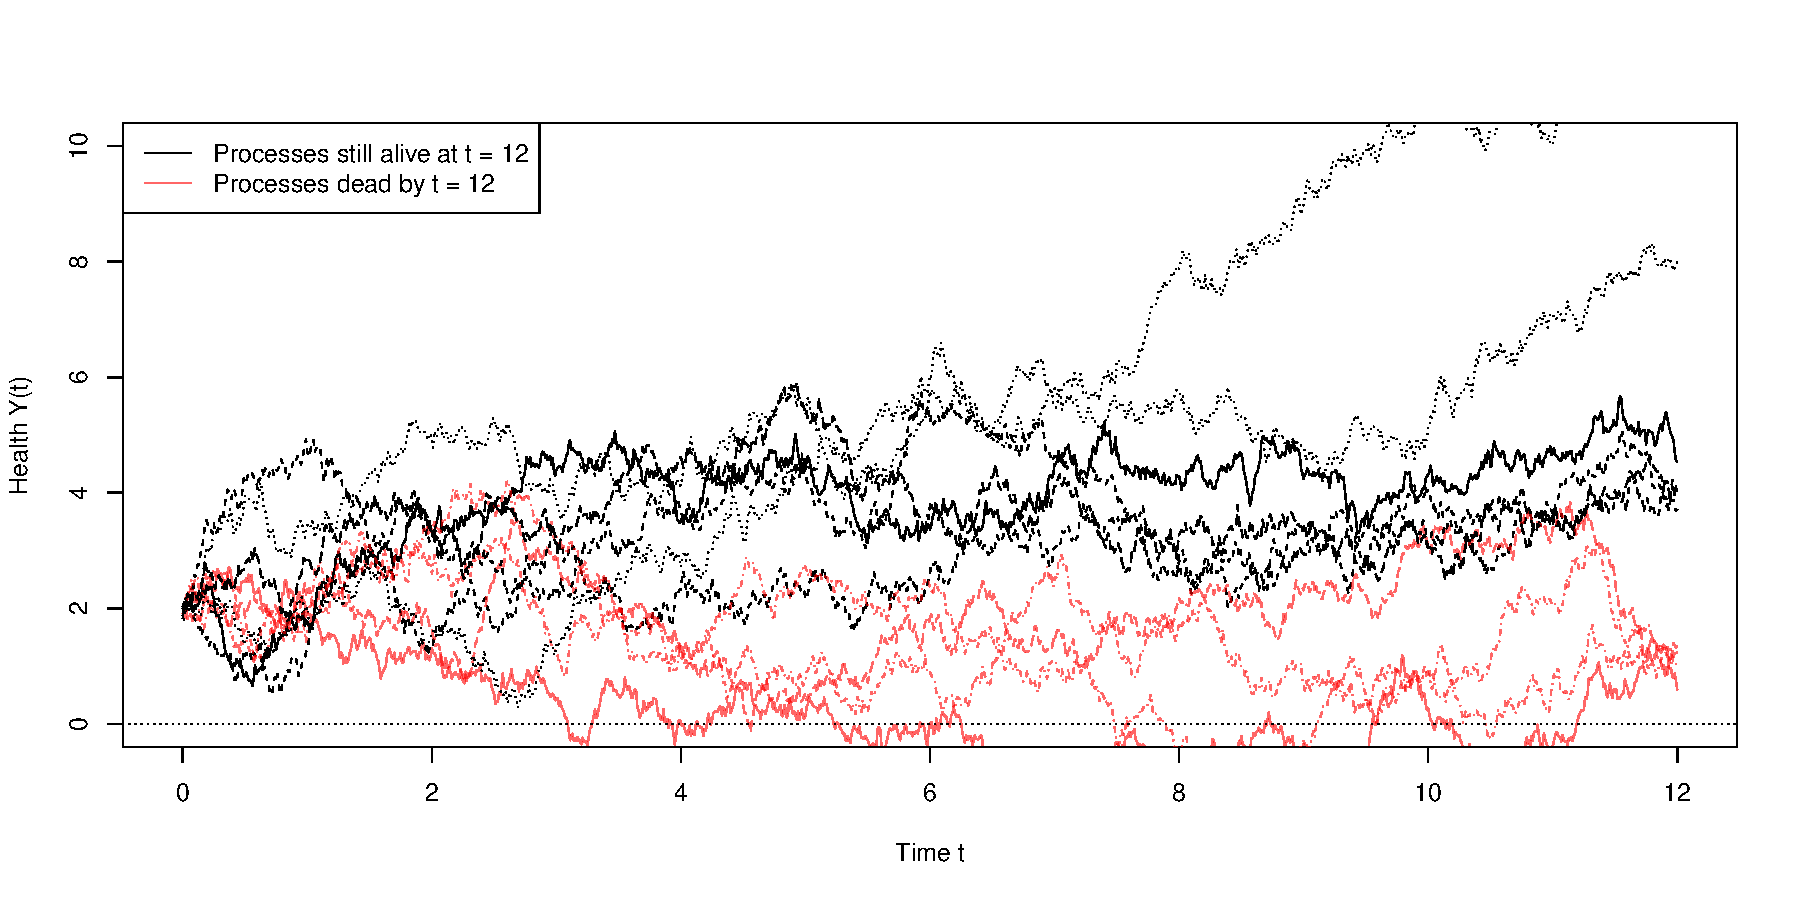
\includegraphics[scale=0.4]{example_wieners6.pdf}
\end{figure}
As mentioned, and as clinicians experience, the survival probability of patients vary, even among those specified as high-risk.
We therefore must look at estimated covariates to see if we can understand this variability.

\subsection{Estimated covariate effects}
The estimated covariate effects are reported in Table \ref{tab:oberthuer-gamma} ($\hat{\bgamma}$) and Table \ref{tab:oberthuer-beta} ($\hat{\bbeta}$), where the estimates in the full model are reported in the middle columns.
We first observe that the boosting algorithm has included both clinical covariates into the model, i.e. the age at diagnosis and the risk indicator.
The full model has also included 8 genes for this training set.
Remember that we centered each column of the covariate matrices, such that the mean across all individuals is (approximately) 0 for each covariate $j$.
%\begin{equation}
%    \overline{x}_j=\frac{1}{n}\sum_{i=1}^n x_{i,j}\approx 0,
%\end{equation}
%\begin{equation}
%    s_j=\frac{1}{n}\sum_{i=1}^n (x_{i,j}-\overline{x}_j)^2\approx 1.
%\end{equation}
%(See a previous section for an explanation of why centering and scaling is important.)
For the gene expressions, this is not particularly important with regards to interpretation, as the scale of these do not lend themselves easily to interpretation.
However, to properly consider the interpretation of the estimated parameters for to the clinical measurements, we should consider these on their original scale.
For example, the covariate corresponding to risk, namely $\gamma_1$, is originally either 0 or 1, depending on the covariate.
After standardizing, these covariates are -0.677 and 1.472, respectively.
The most striking result here is the large size of the estimated parameter corresponding to risk, namely -0.259.
We calculate the drift parameter for those individuals designated as high-risk, and it is
\begin{equation*}
    \mu^{[0]}_{\text{high-risk}}=0.332-0.259\cdot1.472=-0.049,
\end{equation*}
whereas for those designated as low and intermediate risk, it is
\begin{equation*}
    \mu^{[0]}_{\text{low-risk}}=0.332-0.259\cdot-0.677=0.507.
\end{equation*}
The drift for those with high risk is negative, while it is quite positive, for low risk.
Since the age column is standardized, these two drift covariates are the mean drift parameters for each of the groups.
We may check that this holds true for all individuals within the risk groups.
The effect of age is negative, which means that there is some downward effect on the drift as the child's age increases.
This negative effect could also potentially lead to low-risk individuals having an estimated negative drift, if the child is sufficiently old.
This is, however, not the case.
The effect of age is so small as to not impact the sign of the drift.
Because the maximum standardized age is 4.193, the age contribution to drift is bounded below by 
\begin{equation*}
    -0.039\cdot4.193=-0.164.
\end{equation*}
Similarly, there are no high-risk individuals for which the drift will be positive, since the minimum standardized age is -0.724, and so the effect of age is bounded above by
\begin{equation*}
    -0.039\cdot-0.724=0.028.
\end{equation*}
Hence, unfortunately, this means that the model predicts that all high-risk children will eventually die from of neuroblastoma cancer.
This seems to resonate with the fact that these children are indeed characterized as having a high risk of recurrence.
Those not designated as high-risk, on the other hand, have a non-zero probability of not experiencing recurrence.
We calculate it using the formula seen previously, namely
\begin{equation*}
    1-\exp{(-2\cdot y_{0}^{[0]}\cdot\mu_{\text{low-risk}}^{[0]})}=1-\exp{(-2\cdot 1.946\cdot 0.507)}=0.861.
\end{equation*}
We should therefore expect, based on the estimated model, that almost all of the low-risk patients should recover.
Briefly, we also observe that the estimated parameter for the risk covariate is slightly larger, in absolute terms, for the clinical-only FHT model, at -0.371.
We should also consider the gene covariates.
\begin{table}
\caption{Results of estimated clinical coefficients on neuroblastoma data \citep{oberthuer-data}.}
\label{tab:oberthuer-gamma}
\centering
\begin{tabular}{lrr}
\toprule
Clinical covariate & $\hat{\gamma}_j$ (full) & $\hat{\gamma}_j$ (clinical only)\\
\hline
Risk      &  -0.259  &  -0.371 \\
Age       &  -0.039  &       0 \\
\bottomrule
\end{tabular}
\end{table}

We observe that 7 genes have been selected in 27 boosting iterations (see the $\hat{\beta}_j$ column in Table \ref{tab:oberthuer-beta}).
Some effects are estimated to be positive, some to be negative, but all are roughly the same size in absolute terms.
Again, the gene expression measurements have been centered and scaled.
However, a larger parameter does not necessarily mean that the effect of this gene is in general larger than others, as it still depends somewhat on the distribution of these.
We recall e.g. from the simulation chapter that the effect of a change in $\beta_j$ is multiplicative in $\exp(\beta_j)$, and not additive.
We might for example look at gene 5527.
The estimated effect of it is $\hat{\beta}_{5527}=-0.096$.
The maximum observation of this gene after standardization is 2.664.
For a hypothetical observation which has mean values, and thus no effect, for all other genes, but with max effect of this gene, its $\hat{y}_{0}$ will be
\begin{equation*}
    \hat{y}_{0}=\hat{y}_0^{[0]}\cdot\exp(-0.096\cdot2.664)=1.946\cdot0.774=1.506,
\end{equation*}
whereas the null model has an initial level of 1.946.
Hence this gene has quite a large effect on the initial level of this hypothetical observation, and hence its estimated probability of dying increases.

Finally, we consider the estimated gene effects of the genomic-only model, reported in the rightmost column of Table \ref{tab:oberthuer-beta}.
Only four genes are selected in the model, and two of these are not selected in the somewhat larger full model, namely gene 3191 and 5307.
It turns out that these are highly correlated with the risk indicator.
For gene 3191 the correlation is 0.532, and for 5307 it is -0.597.
The positive correlation for gene 3191 means that if a child has a large measured gene effect, the likelihood of it being diagnosed as high risk is larger than if it has a mean effect of this gene.
Conversely, since the correlation for gene 5307 is highly negative, it is likely that a child with a high value of this gene has a low risk indicator, compared to if it has a mean effect of this gene.
We show a scatterplot of these genes and the risk indicator in Figure \ref{fig:gene-corr}.

\begin{figure}
\caption{Scatterplots of genes 3191 (top) and 5307 (bottom) with the risk indicator for the neuroblastoma data set.}
\label{fig:gene-corr}
\centering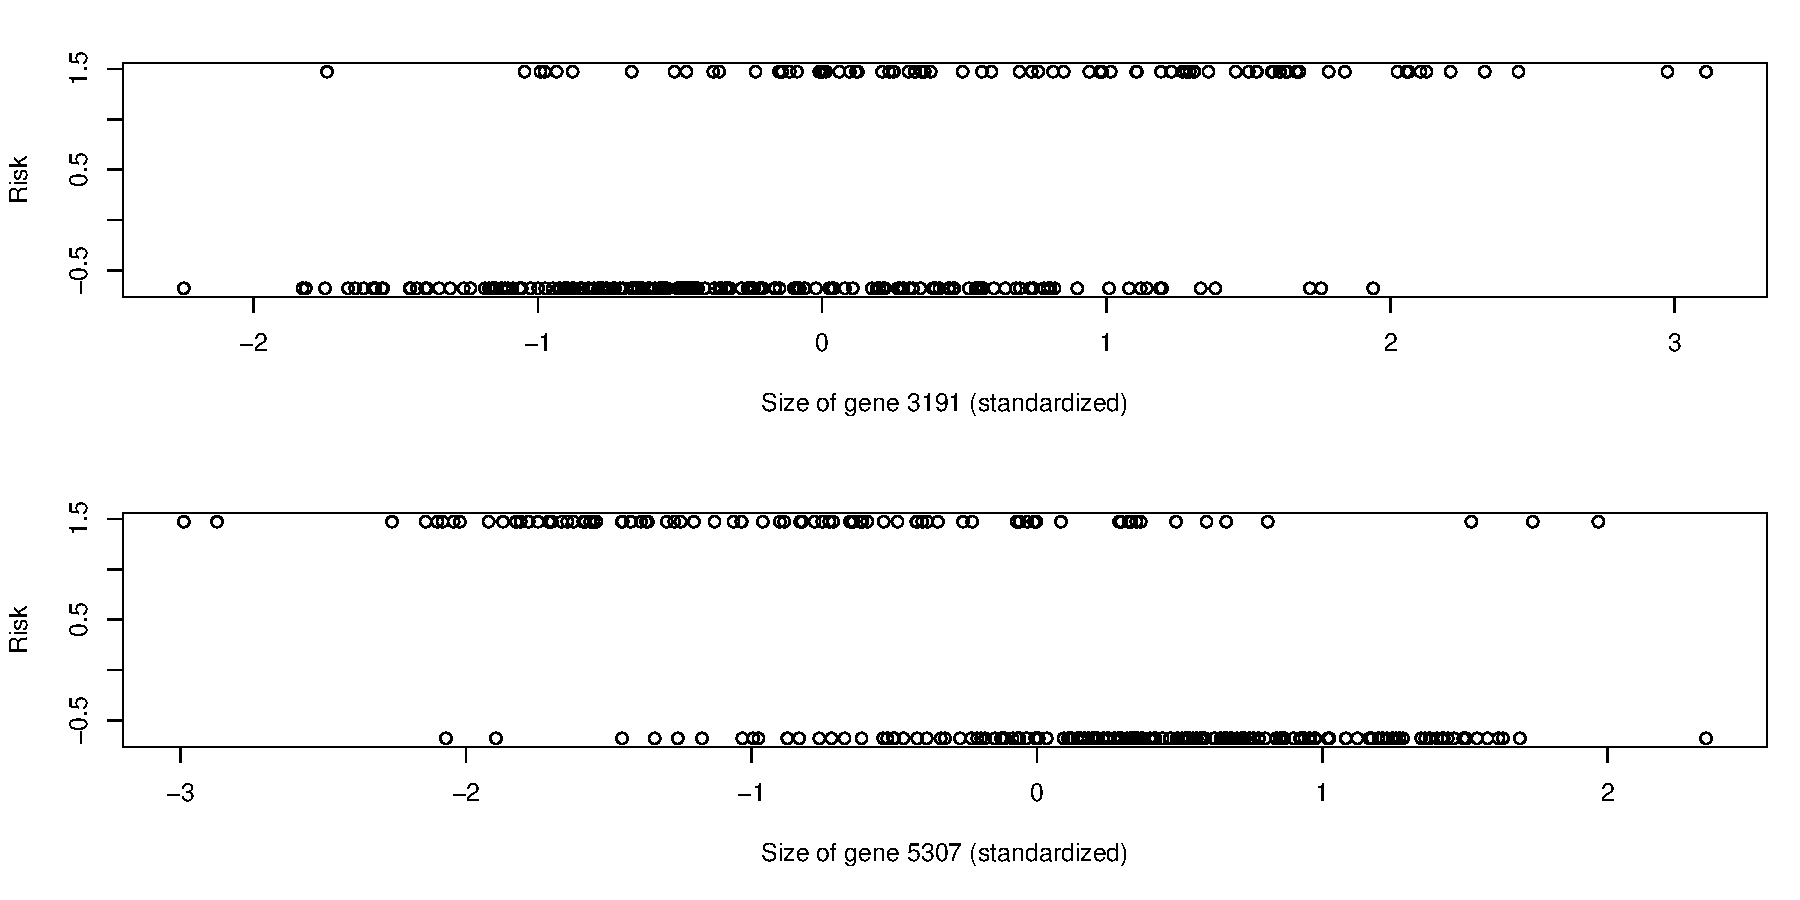
\includegraphics[scale=0.4]{gene_correlations.pdf}
\end{figure}


\begin{table}
\caption{Results of estimated gene coefficients on neuroblastoma data \citep{oberthuer-data}.}
\label{tab:oberthuer-beta}
\centering
\begin{tabular}{lrr}
\toprule
Gene $j$      & $\hat{\beta}_j$ (full) & $\hat{\beta}_j$ (genomic only)\\
\hline

Gene 1447 & -0.064 & -0.093 \\
Gene 2442 &  0.038 &      0 \\
Gene 2783 & -0.024 &      0 \\
Gene 3191 &      0 & -0.093 \\
Gene 5307 &      0 &  0.046 \\
Gene 5527 & -0.096 & -0.201 \\
Gene 5725 & -0.011 &      0 \\
Gene 6901 &  0.013 &      0 \\
Gene 7523 & -0.023 &      0 \\
\bottomrule
\end{tabular}
\end{table}

\subsection{Measurement results on the test set}
We now examine the results of the estimated models on the test set.
The test set in this split consists of 91 individuals, of which 14 have experienced recurrence.

\subsubsection{Difference of deviance}
We calculate the difference in deviance for the estimated FHT model.
As explained in Section \ref{sec:deviance}, the difference of deviance is twice the difference between the log-likelihood for an estimated model which includes covariates, and a model without covariates.
The performance of a model is good when the difference in deviance is small (i.e. negative with a large absolute value).
We obtain a difference of deviance of -108.9 for the full FHT model.
It means that under the assumption that the FHT model is true, a lot of variation is explained by covariates.
For this test set, the full model is in fact beaten by the genomic model, with difference of deviance of -108.9 and -129.7, respectively.
The clinical model is worse, but still better than the null model, with a difference of deviance at -26.2.

\begin{table}
\caption{Difference of deviance with FHTBoost with a fixed intercept, on a single split of the neuroblastoma data \citep{oberthuer-data}.}
\label{tab:deviances}
\centering
\begin{tabular}{lr}
\toprule
Boosting type & Difference of deviance \\
\hline
Full                   & -108.9 \\
Clinical ($y_0$) only  &  -26.2 \\
Genomic ($\mu$) only   & -129.7 \\
\bottomrule
\end{tabular}
\end{table}

\subsection{Brier score}
We now calculate Brier scores (Section \ref{sec:brier}) on each observation in the test set with each FHT model, see Figure \ref{fig:brier-FHT} for a graphic display of these.
Interestingly, the full FHT model is quite consistently better than the genomic model, i.e. it is better per observation in the Brier score, even though it achieves a worse difference of deviance.
Furthermore, the Brier score of the full FHT model is almost equal to the clinical one in some parts, except in the middle, from 3 to 7 years, where the full model is somewhat better.
It is perhaps easiest to compare the performance if we have a number, and we get that by calculating the integrated Brier score, explained in subsection \ref{subsec:integrated-brier}, and which is effectively the average Brier score over a given range of time, in this case the times from the entire test set.
We find that the integrated Brier score for the full FHT model is 0.051.
The genomic model attains an integrated Brier score of 0.085, while the clinical attains 0.057.
For reference, the estimated FHT null model achieves 0.122, which is almost the double.

\begin{figure}
\caption{Brier scores for FHT models.}
\label{fig:brier-FHT}
\centering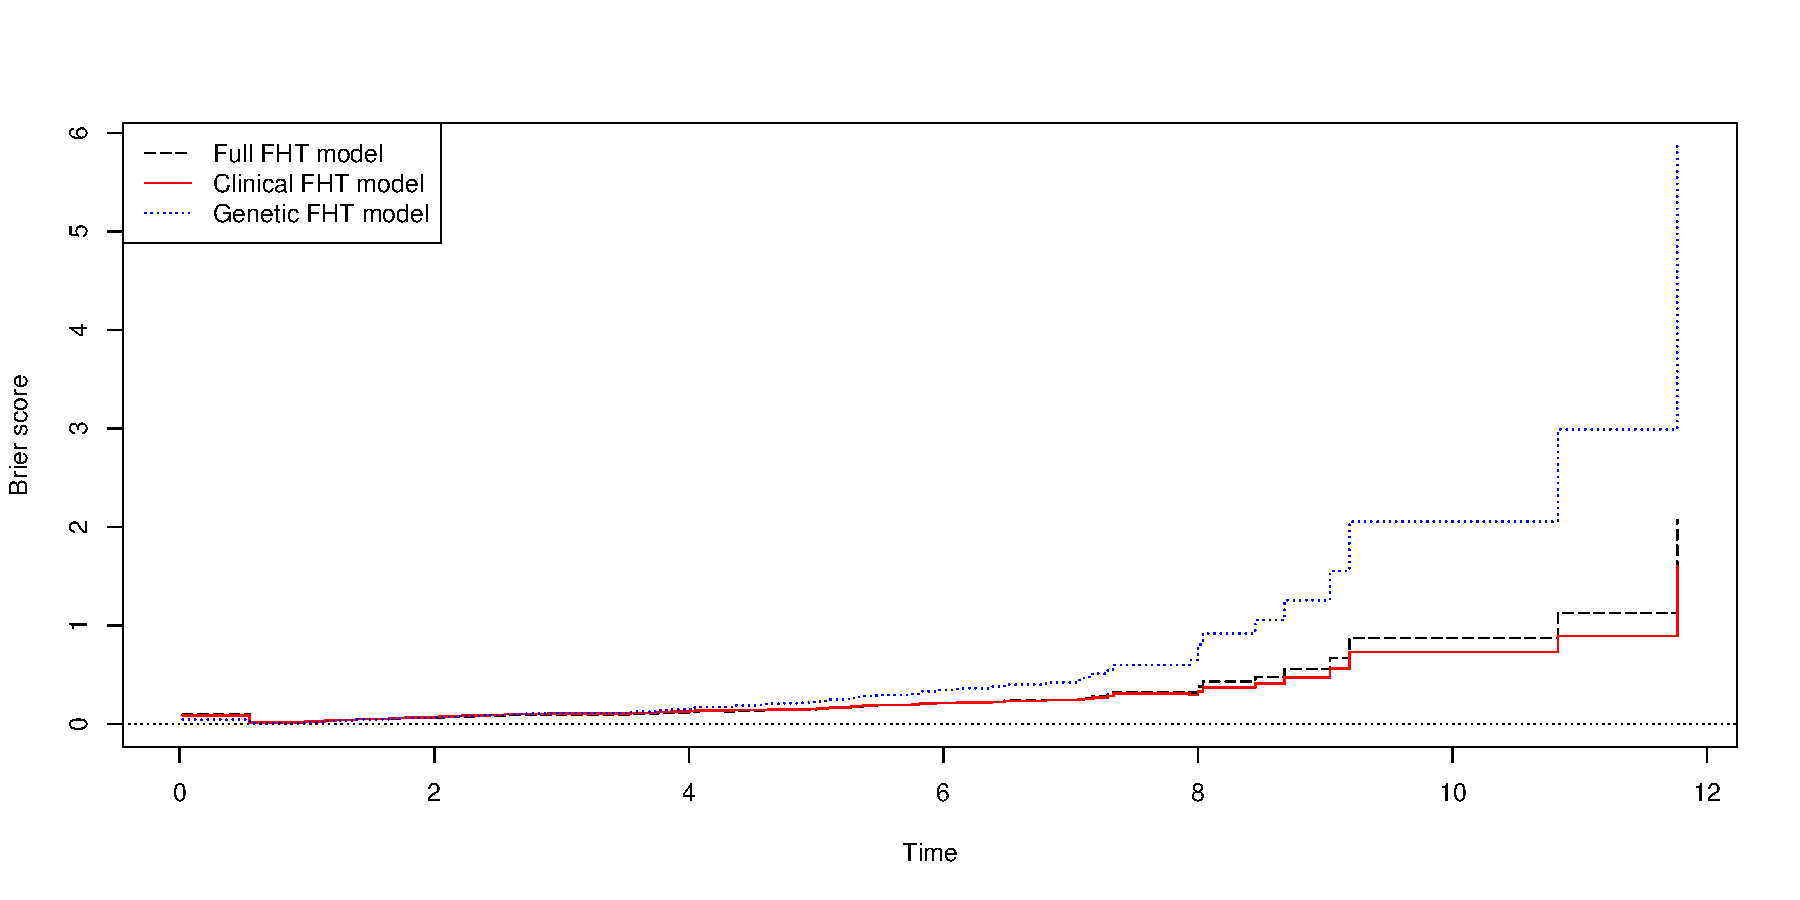
\includegraphics[scale=0.4]{brier_FHT.pdf}
\end{figure}

A comparison of the Brier score for the full FHT model and the regular Cox model can be seen in Figure \ref{fig:brier-cox-both}.
We observe that the Cox model performs slightly better at the beginning, but at the end, the FHT model has better predictive performance.
Note, however that large part of the additional error of the Cox model refers to the right part of the error curve (see Figure \ref{fig:brier-FHT}), where the computations are more unstable due to the reduced number of events (larger proportion of censored data).
The estimated CoxBoost model attains 0.067, and so it is beaten by the full FHT model.
However, the mandatory Cox model achieves an integrated Brier score of 0.044.

\begin{figure}
\caption{Brier scores on a single split of the test set of the neuroblastoma data, for an estimated CoxBoost survival model and a full estimated FHT model.}
\label{fig:brier-cox-both}
\centering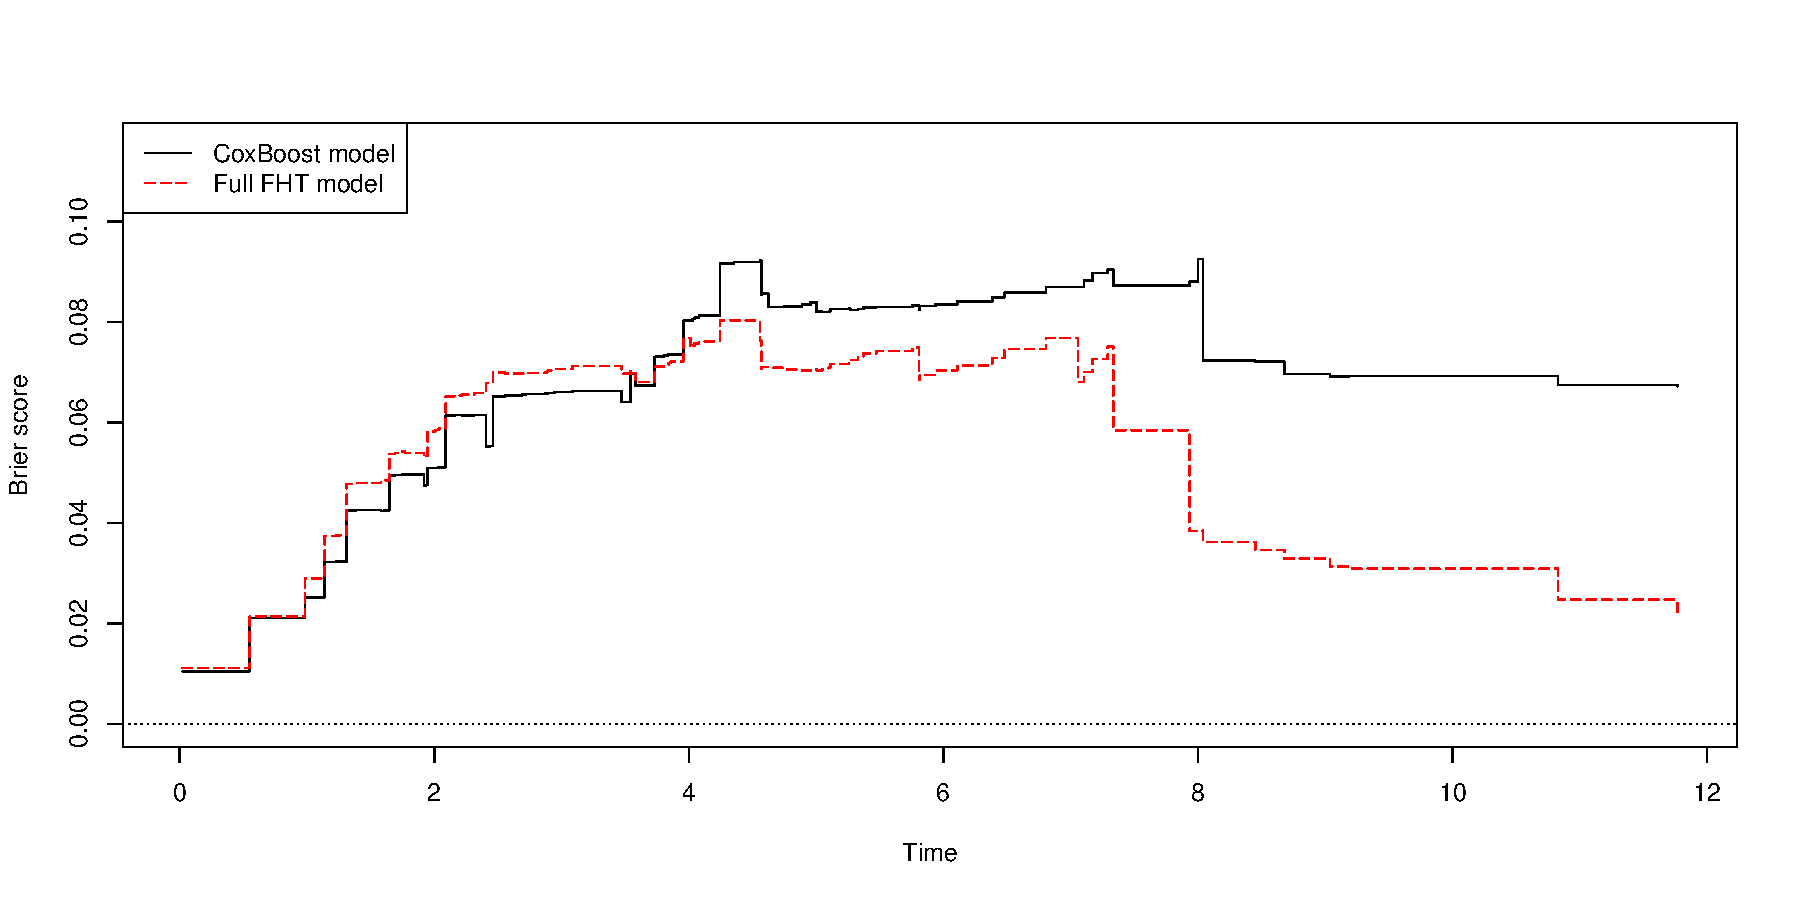
\includegraphics[scale=0.4]{brier_cox_both.pdf}
\end{figure}

%\begin{figure}
%\caption{Brier scores for Cox and Cox mandatory model.}
%\label{fig:brier-cox-mandatory}
%\centering
%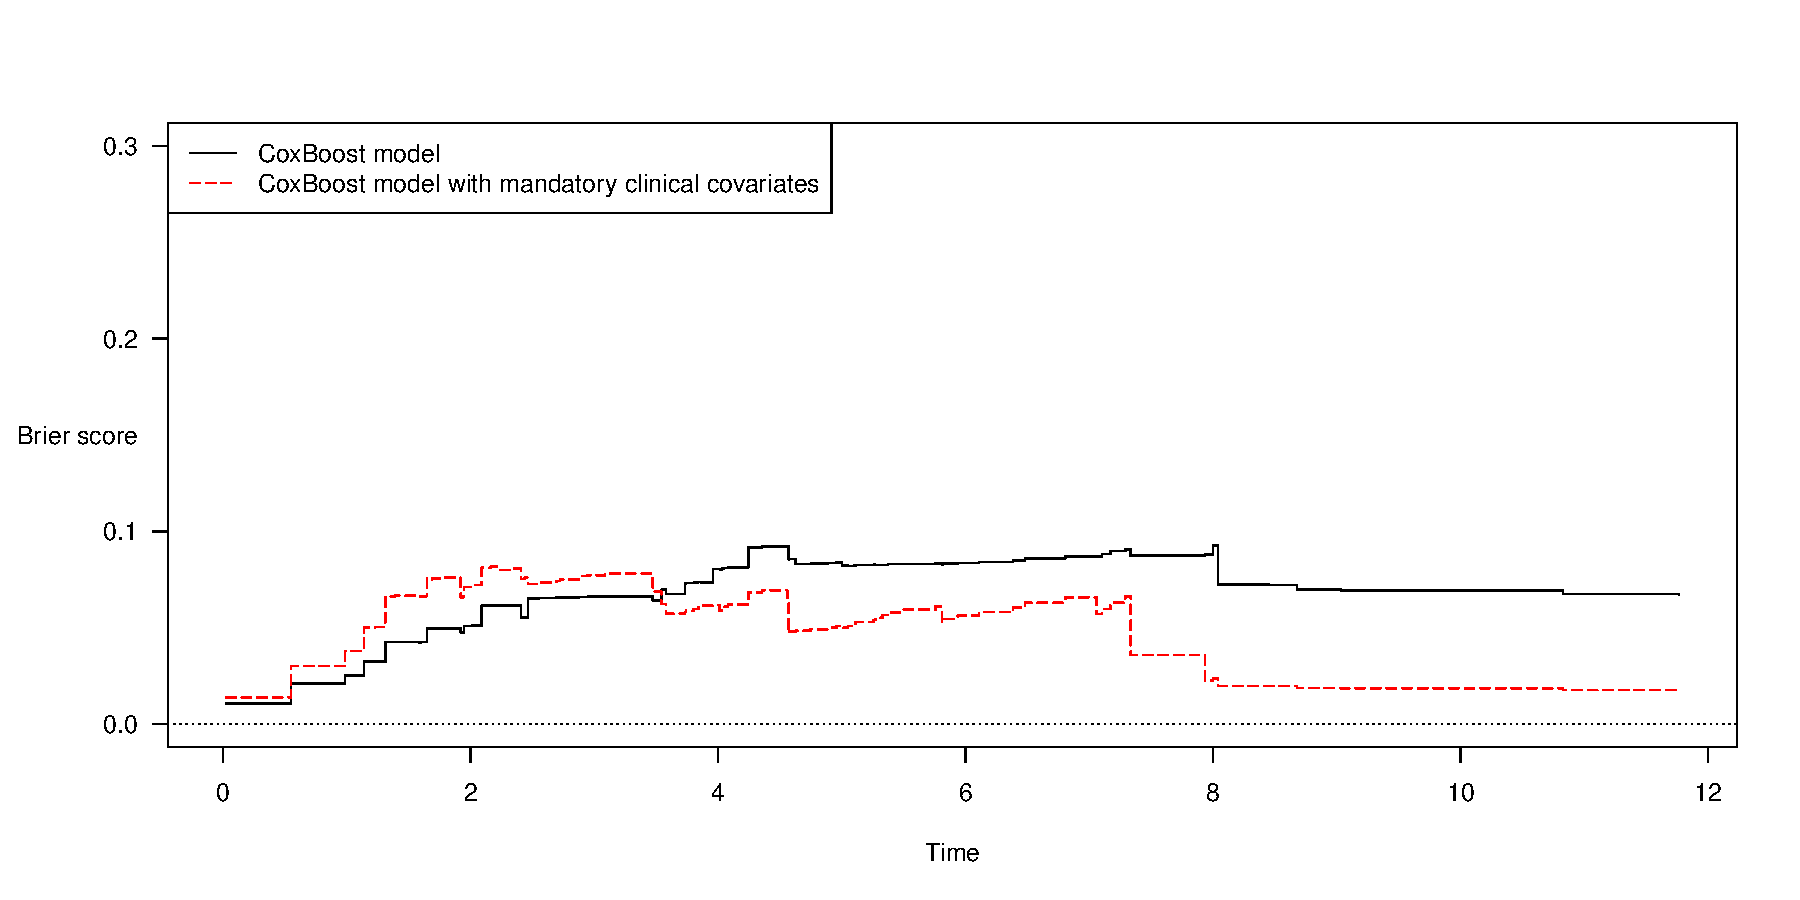
\includegraphics[scale=0.4]{brier_cox_mandatory.pdf}
%\end{figure}

%\todo[inline]{Cite these packages! I think cite(package) in R}


\section{Results of 100 train/test splits}
As mentioned above, we generate 99 additional splits into training and test sets, for a total of 100.
We proceed in the same manner on the single split, i.e. estimating parameters by first finding an optimal number of iterations $\mstop$, and then running the boosting algorithm for that amount of iterations.
Finally, we use the estimated model on the test set and calculate the evaluation measures.

\subsection{Difference of deviance in FHT models}
Figure \ref{fig:neuroblastoma-deviances} shows a boxplot of the difference of deviance across all 100 splits of training and test sets.
The main measure of interest is the mean for each, and it is -51.0 for the full model, -23.4 for the clinical model, and -40.3 for the genomic model.
The full FHT model has the best mean value here, which should be expected, as it can include both clinical and genomic covariates.

\begin{figure}
\caption{Boxplot for difference in deviance for different variants of the FHT model.}
\label{fig:neuroblastoma-deviances}
\centering
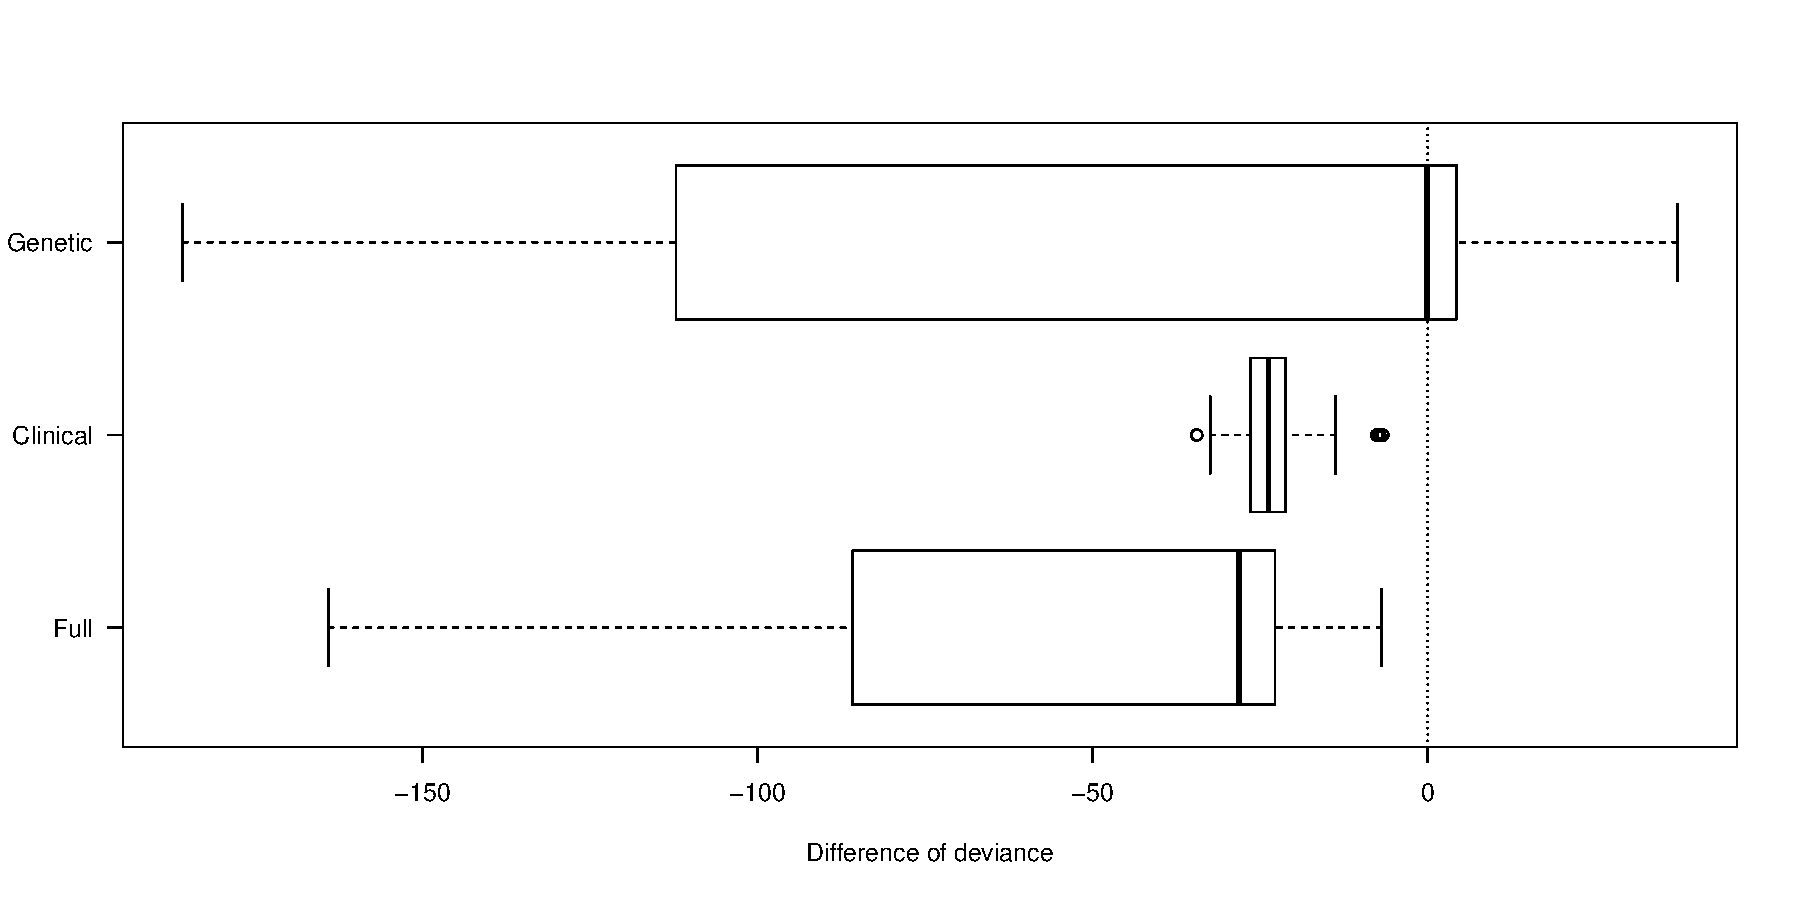
\includegraphics[scale=0.4]{deviance_FHT.pdf}
\end{figure}

%These deviances look a bit strange, at least the box for the full model, and the box for the genomic model.
%The median looks to be very strangely positioned, all the way to the right of the boxes.
%We plot histograms of these two to consider why.
%See Figure \ref {fig:neuroblastoma-deviances-histo}.
%The reason turns out to be that they are quite bimodal in their distribution.
%Both have large peaks around 0, and both have smaller and wider peaks more to the left.
%We see that the full model consistently improves performance with covariates, i.e., has a negative difference of deviance.
%This resonates with the fact that the clinical model also improves over the null model.
%However, the genomic model very often does not improve on the null model.
%Although, its most extreme values are in cases where the difference of deviance is very small, and so these are cases where the genomic model outperforms the full model.

%\begin{figure}
%\caption{Histogram of difference of deviance for the genomic model and the full model.}
%\label{fig:neuroblastoma-deviances-histo}
%\centering
%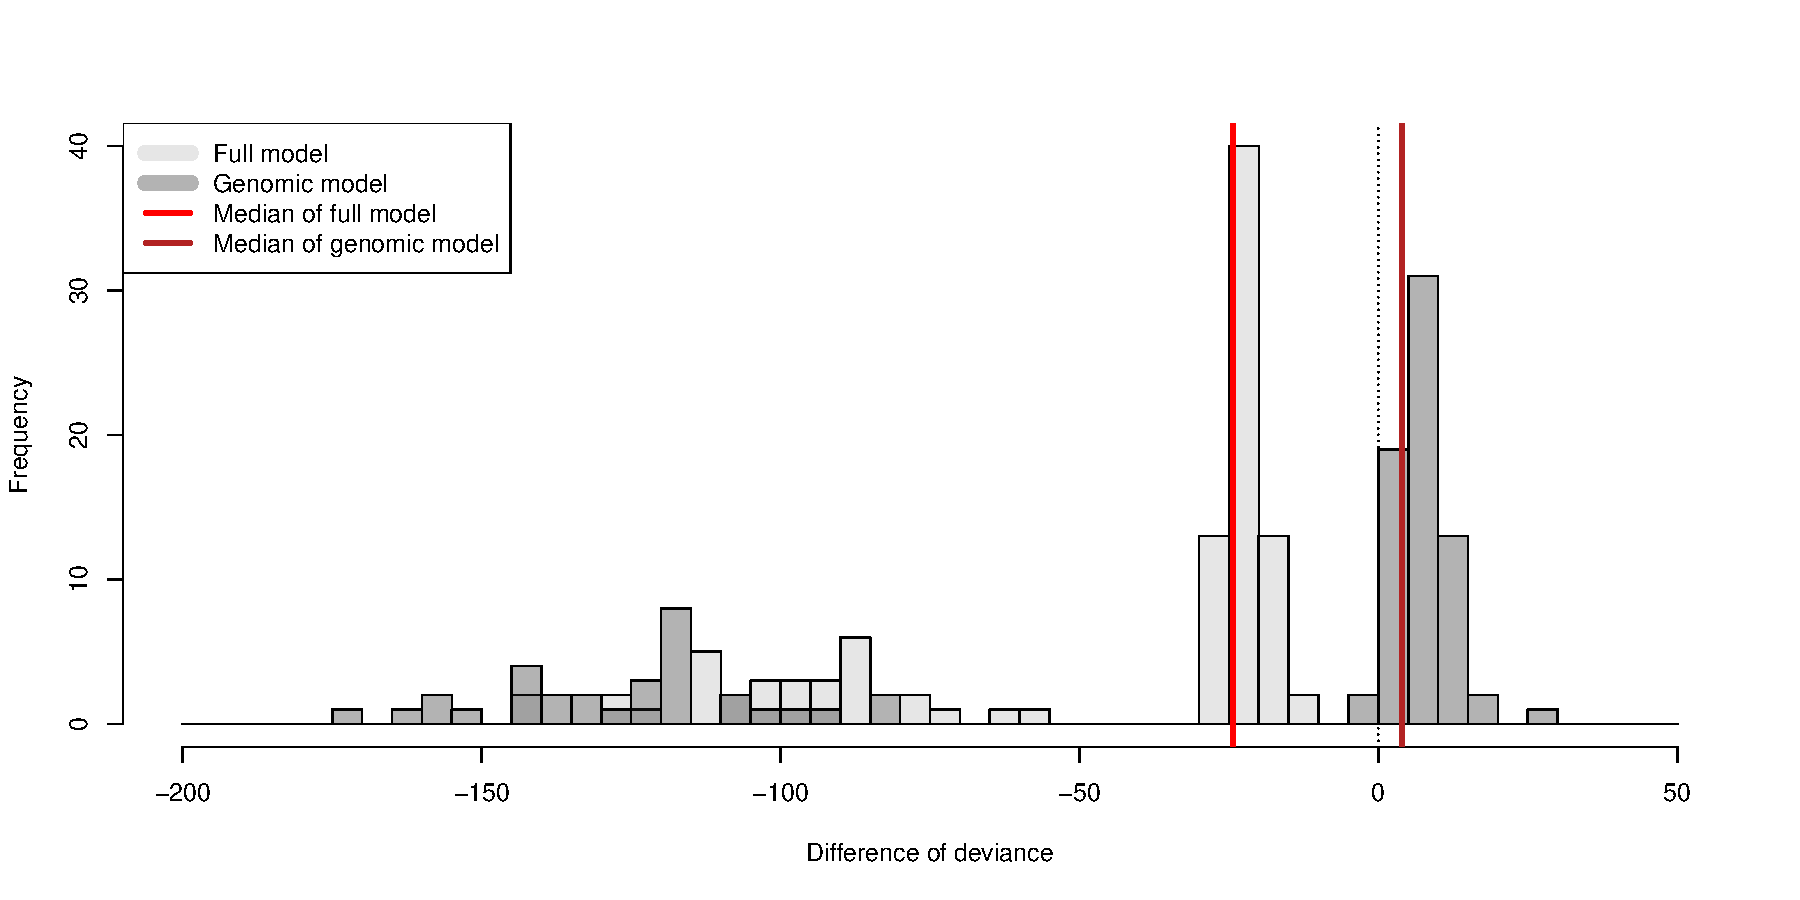
\includegraphics[scale=0.4]{deviances_histogram.pdf}
%\end{figure}


\subsection{Integrated Brier scores}
We now calculate the integrated Brier scores for all 100 splits, for all of the mentioned methods.
A boxplot can be seen in Figure \ref{fig:neuroblastoma-integrated-brier}, and Table \ref{tab:mean-brier} reports the mean of these.
\begin{figure}
\caption{Boxplot of integrated Brier scores.}
\label{fig:neuroblastoma-integrated-brier}
\centering
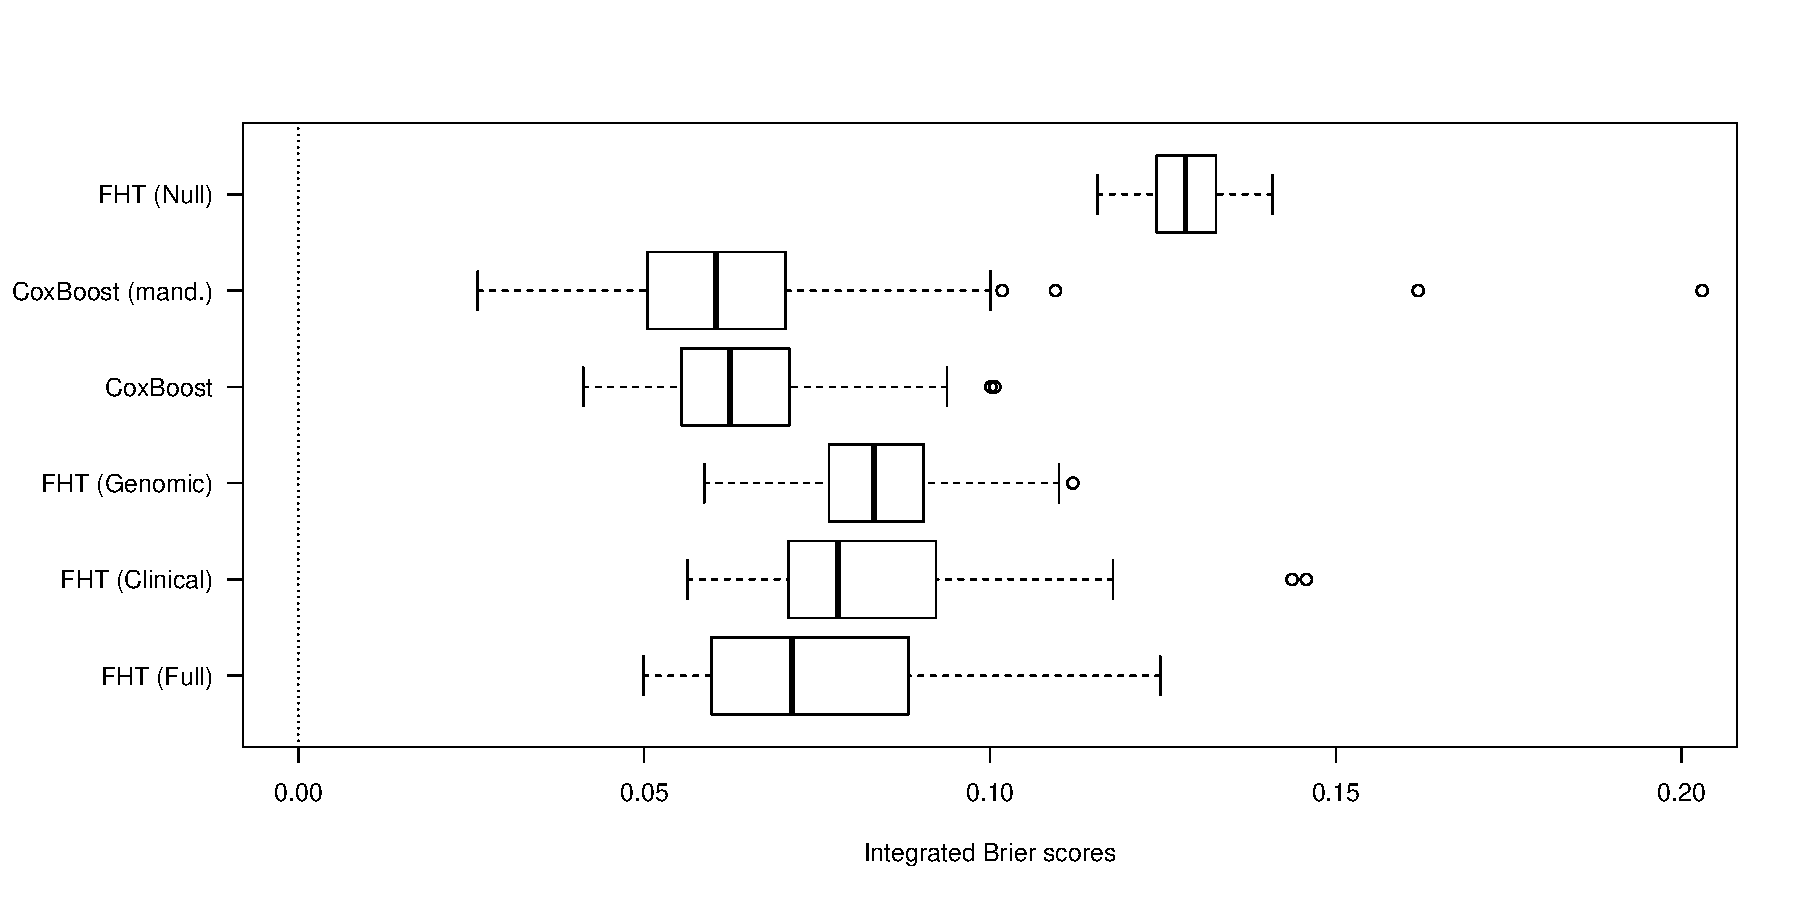
\includegraphics[scale=0.4]{integrated_brier_boxplot.pdf}
\end{figure}
\begin{table}
\caption{Mean integrated Brier score on all splits of the neuroblastoma data \citep{oberthuer-data}.}
\label{tab:mean-brier}
\centering
\begin{tabular}{lr}
\toprule
Model                      & Mean integrated Brier score \\
\hline
FHT Full                   & 0.074 \\
FHT Clinical ($y_0$) only  & 0.083 \\
FHT Genomic ($\mu$) only   & 0.084 \\
Cox regular                & 0.064 \\
Cox mandatory              & 0.069 \\
\bottomrule
\end{tabular}
\end{table}
The full FHT model performs best of the FHT models, which again should be the case, as it can use all covariates.
It is, however, beaten by both Cox models, but only slightly.
This is encouraging, as these results show that regression with FHT models can compete with Cox regression, also on realistic and high-dimensional data.